\chapter{Plano de trabalho e conclusões}\label{chap:chap3}

Neste capítulo apresenta-se o plano de trabalho a ser realizado durante o desenvolvimento do projeto de dissertação através do diagrama de Gantt, com os períodos de tempo previstos para a sua execução, de acordo com os objetivos propostos no~\ref{chap:intro}, secção~\ref{sec:object}. São também referenciadas as ferramentas e tecnologias necessárias para o desenvolvimento deste projeto e uma pequena conclusão.

\section{Plano de trabalho}

Nesta secção é apresentado na figura~\ref{fig:gantt} o diagrama de Gantt com as tarefas previstas e com a respetiva distribuição das mesmas ao longo do tempo definido para o desenvolvimento do projeto de dissertação.  

\begin{figure}[h]
\scalebox{1}{
\begin{gantt}[xunitlength=0.5cm,fontsize=\small,titlefontsize=\small]{10}{18}
%\begin{gantt}{10}{18}
	\begin{ganttitle}
	    \titleelement{Feb}{3}
	    \titleelement{Mar}{4}
	    \titleelement{Apr}{5}
	    \titleelement{May}{4}
	    \titleelement{Jun}{2}
	\end{ganttitle}
	\begin{ganttitle}
	      \numtitle{2}{1}{4}{1}
	      \numtitle{1}{1}{4}{1}
	      \numtitle{1}{1}{5}{1}
	      \numtitle{1}{1}{4}{1}
	      \numtitle{1}{1}{2}{1}
	    \end{ganttitle}
	\ganttbar[color=red]{Implemetação sistemas acesso às imagens}{0}{2}
	\ganttbar[color=red]{Familiarização com ferramentas de trabalho }{1}{2}
	\ganttbar[color=red]{Especificação do sistema a implementar}{2}{2}
	\ganttbar[color=orange]{Desenvolvimento da primeira versão do modelo}{4}{3}
	\ganttbarcon[color=orange]{Desenvolvimento da segunda versão do modelo}{7}{4}
	\ganttbar[color=yellow]{Extensão do TweeProfiles}{11}{4}
	\ganttbar[color=green]{Escrita da Dissertação}{14}{4}
	\ganttbar[color=cyan]{Criação e actualização do website}{0}{18}

\end{gantt}
}
\caption{Diagarama de Gantt com plano de trabalho}
\label{fig:gantt}
\end{figure}

\begin{description}
\item[Implementação sistemas acesso ás imagens:] Para a realização deste projeto será necessário realizar a recolha dos \textit{urls} das imagens partilhadas através do serviço Twitter e o armazenamento das respetivas imagens para que possam posteriormente ser utilizadas para o objetivo desta dissertação referido no capítulo~\ref{chap:intro}, secção~\ref{sec:object}.A duração prevista para esta etapa é de \textbf{duas semanas}.

\item[Familiarização com ferramentas de trabalho:] Nesta fase inicial, é necessário fazer uma avaliação e o estudo das ferramentas e do ambiente de desenvolvimento para as fases seguinte. A duração prevista para esta etapa é de \textbf{duas semana}.

\item[Especificação do sistema a implementar: ] Em paralelo com a etapa anterior, dá-se início à especificação do sistema que irá analisar as imagens e ser capaz de apresentar \textit{clusters} das mesmas. Será também definida a estratégia de ataque ao problema. A duração prevista para esta etapa é de cerca de \textbf{duas semanas}.

\item[Desenvolvimento do sistema :] Esta etapa encontra-se dividida em duas sub-etapas para a implementação do sistema a desenvolver. Enquanto que a segunda  Esta etapa terá uma duração total prevista de \textbf{sete semanas}

\begin{enumerate}
\item \textbf{Primeira versão: } Que seja capaz de realizar a tarefa de \textit{clustering} recorrendo a apenas algumas imagens. Esta Sub-tarefa terá uma duração prevista de \textbf{três semanas}
\item \textbf{Segunda versão: } Que seja capaz de realizar a tarefa de \textit{clustering} recorrendo a uma base de dados maior. Esta Sub-tarefa terá uma duração prevista de \textbf{quatro semanas}
\end{enumerate}

\item[Extensão do TweeProfiles: ] Esta etapa refere-se ao processo de implementação do sistema desenvolvido na etapa anterior, em que se procederá à extensão da ferramenta TweeProfiles~\citet{Cunha2013} com teste. Esta etapa tem uma duração prevista de cerca de \textbf{quatro semanas}.  

\item[Escrita da Dissertação: ] Após todos os testes realizados e feita a análise dos resultados obtidos, será realizado a última etapa, que corresponde à escrita do documento final. que deverá descrever todo o trabalho desenvolvido ao longo do semestre e as conclusões retiradas. Esta etapa tem uma duração prevista de cerca de \textbf{quatro semanas}.

\item[Criação e atualização da página web: ] Esta será uma tarefa continua ao longo do desenvolvimento da dissertação, em que será criada uma pagina web com informação relativa ao projeto, e que será constantemente atualizada com os respetivos desenvolvimentos.
\end{description}


\section{Ferramentas de apoio}

Nesta secção faz-se referência às ferramentas e tecnologias utilizadas para o desenvolvimento do trabalho.

Todos os tweets estão alojados numa base de dados Mongodb. Para acesso à informação será utilizada a linguagem Python, mais especificamente, através da utilização da biblioteca Pymongo. Será também necessário recorrer a uma base de dados relacional PostgreSQL para o armazenamento dos endereços de acesso à fonte das fotografias e de outras informações pertinentes que permita uma pesquisa facilmente filtrada. 

%Todos os tweets estão alojados numa base de dados Mongodb, sendo possível recorrer à informação armazenada recorrendo à linguagem Python, mais precisamente com a biblioteca Pymongo. Será também necessário a utilização de uma base de dados relacional PostgreSQL para o armazenamento dos endereços à fonte das fotografias e de outras informações pertinentes que facilite a filtragem das mesmas. 

Para o desenvolvimento do sistema de processamento das imagens será utilizado a ferramenta livre OpenCV.


\section{Conclusão}

Este relatório foi realizado com o intuito de preparar a realização do projeto de dissertação. Assim, primeiramente é apresentada uma introdução com a descrição do tema, das motivações e objetivos deste trabalho. De seguida, o capítulo~\ref{chap:estarte} apresenta o estado da arte, onde foi realizada a revisão bibliográfica, recorrendo a pesquisa de livros e artigos científicos, informação esta que se revelou importante para a compreensão das tarefas necessárias a realizar, bem como dos conteúdos a dominar. Para além disto, este capitulo faz uma introdução teórica a alguns conteúdos que são necessários dominar. Por fim, foi apresentado o diagrama de Gantt que descreve as tarefas a realizar e a correspondente duração, e ainda, as ferramentas necessárias para o desenvolvimento do projeto.


%Este relatório foi realizado com o intuito de preparar a realização do projeto de dissertação. Assim, o primeiro passo foi a apresentação de uma breve introdução com a descrição do tema, das motivações e objetivos deste trabalho. Já o capítulo~\ref{chap:estarte}, apresenta o estado da arte, onde foi realizada a revisão bibliográfica, recorrendo a pesquisa de livros e artigos científicos, informação esta que se revelou importante para a compreensão das tarefas necessárias a realizar, bem como dos conteúdos a dominar. Para além disto, este capitulo faz uma introdução teórica a alguns conteúdos que são necessários dominar.Por fim, foi apresentado o diagrama de Gantt que descreve as tarefas a realizar e a correspondente duração e as ferramentas que serão utilizadas para o desenvolvimento do projeto.

Após a finalização deste relatório final, conclui-se que este projeto possui suporte cientifico e tecnológico para que seja concretizado. 



% % % % % % % % % % % % % % % % % % % % % % % % % % % % % % % % % % % % % % % % % % % % %
%Apresenta-se de seguida um exemplo de equação, completamente fora do contexto:
%\begin{eqnarray}
%CIF_1: \hspace*{5mm}F_0^j(a) &=& \frac{1}{2\pi \iota} \oint_{\gamma} \frac{F_0^j(z)}{z - a} dz\\
%CIF_2: \hspace*{5mm}F_1^j(a) &=& \frac{1}{2\pi \iota} \oint_{\gamma} \frac{F_0^j(x)}{x - a} dx \label{eq:cif}
%\end{eqnarray}
%
%Na Equação~\ref{eq:cif} lorem ipsum dolor sit amet, consectetuer
%adipiscing elit. Suspendisse tincidunt viverra elit. Donec tempus
%vulputate mauris. Donec arcu. Vestibulum condimentum porta
%justo. Curabitur ornare tincidunt lacus. Curabitur ac massa vel ante
%tincidunt placerat. Cras vehicula semper elit. Curabitur gravida, est
%a elementum suscipit, est eros ullamcorper quam, sed cursus velit
%velit tempor neque. Duis tempor condimentum ante. Nam
%sollicitudin. Vestibulum adipiscing, orci eu tempor dapibus, risus
%sapien porta metus, et cursus leo metus eget nibh. 
%
%\section{Secção Exemplo}
%
%A arquitectura do visualizador assenta sobre os seguintes conceitos
%base~\citep{kn:ZPMD97}: 
%
%\begin{itemize}
%\item \textbf{Componentes} --- Suspendisse auctor mattis augue \emph{push};
%\item \textbf{Praesent} --- Sit amet sem maecenas eleifend facilisis leo;
%\item \textbf{Pellentesque} --- Habitant morbi tristique senectus et netus.
%\end{itemize}
%
%\subsection{Exemplo de Figura}
%
%É apresentado na Figura~\ref{fig:arch} da página~\pageref{fig:arch} um
%exemplo de figura flutuante que deverá ficar no topo da página.
%
%\begin{figure}[t]
%  \begin{center}
%    \leavevmode
%    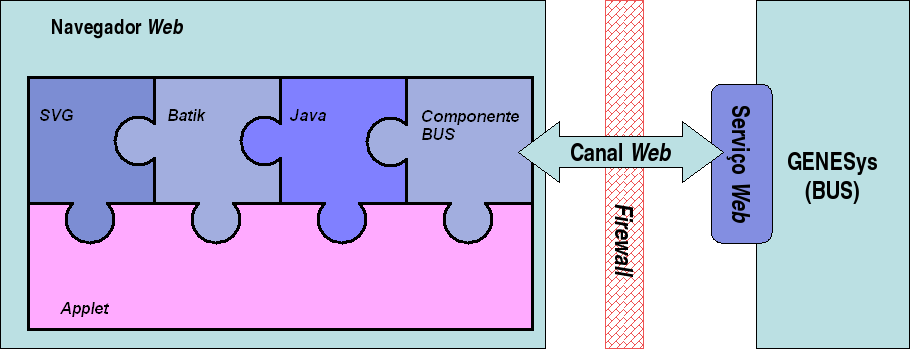
\includegraphics[width=0.86\textwidth]{puzzle}
%    \caption{Arquitectura da Solução Proposta}
%    \label{fig:arch}
%  \end{center}
%\end{figure}
%
%Loren ipsum dolor sit amet, consectetuer adipiscing elit. 
%Praesent sit amet sem. Maecenas eleifend facilisis leo. Vestibulum et
%mi. Aliquam posuere, ante non tristique consectetuer, dui elit
%scelerisque augue, eu vehicula nibh nisi ac est. Suspendisse elementum
%sodales felis. Nullam laoreet fermentum urna. 
%
%
%\subsection{Exemplo de Tabela}
%
%É apresentado na Tabela~\ref{tab:exemplo} um exemplo de tabela
%flutuante que deverá ficar no topo da página.
%
%\begin{table}[t]
%  \centering
%  \caption{Tabela Exemplo}
%\begin{tabular}{|c|r@{.}lr@{.}lr@{.}l||r|}
%	\hline
%\multicolumn{8}{|c|}
%	{\rule[-3mm]{0mm}{8mm}Iteração $k$ de $f(x_n)$} \\
%\textbf{\em k}
%	& \multicolumn{2}{c}{$x_1^k$}
%	& \multicolumn{2}{c}{$x_2^k$}
%	& \multicolumn{2}{c||}{$x_3^k$}
%	& comentários \\ \hline \hline
%0   & -0&3                 & 0&6                 &  0&7   & - \\
%1   &  0&47102965 & 0&04883157 & -0&53345964  & $\delta<\epsilon$ \\
%2   &  0&49988691 & 0&00228830 & -0&52246185  & $\delta < \varepsilon$ \\
%3   &  0&49999976 & 0&00005380 & -0&523656   &   $N$ \\
%4   &  0&5                 & 0&00000307 & -0&52359743  & \\
%\vdots	& \multicolumn{2}{c}{\vdots}
%	& \multicolumn{2}{c}{$\ddots$}
%	& \multicolumn{2}{c||}{\vdots}  & \\
%7   &  0&5   & 0&0    & \textbf{-0}&\textbf{52359878}
%		 & $\delta<10^{-8}$ \\ \hline
%\end{tabular}
%  \label{tab:exemplo}
%\end{table}
%

